\documentclass[12pt, spanish]{article}
\usepackage[spanish]{babel}
\selectlanguage{spanish}
%\usepackage{natbib}
\usepackage{url}
\usepackage[utf8x]{inputenc}
\usepackage{graphicx}
\graphicspath{{images/}}
\usepackage{parskip}
\usepackage{fancyhdr}
\usepackage{vmargin}
\usepackage{multirow}
\usepackage{float}
\usepackage{chngpage}

\usepackage{amsfonts}

\usepackage{subcaption}

\usepackage{hyperref}
\usepackage[
    type={CC},
    modifier={by-nc-sa},
    version={4.0},
]{doclicense}

\hypersetup{
    colorlinks=true,
    linkcolor=blue,
    filecolor=magenta,
    urlcolor=cyan,
}

% para codigo
\usepackage{listings}
\usepackage{xcolor}



%% configuración de listings

\definecolor{listing-background}{HTML}{F7F7F7}
\definecolor{listing-rule}{HTML}{B3B2B3}
\definecolor{listing-numbers}{HTML}{B3B2B3}
\definecolor{listing-text-color}{HTML}{000000}
\definecolor{listing-keyword}{HTML}{435489}
\definecolor{listing-identifier}{HTML}{435489}
\definecolor{listing-string}{HTML}{00999A}
\definecolor{listing-comment}{HTML}{8E8E8E}
\definecolor{listing-javadoc-comment}{HTML}{006CA9}

\lstdefinestyle{eisvogel_listing_style}{
  language         = c++,
%$if(listings-disable-line-numbers)$
%  xleftmargin      = 0.6em,
%  framexleftmargin = 0.4em,
%$else$
  numbers          = left,
  xleftmargin      = 0em,
 framexleftmargin = 0em,
%$endif$
  backgroundcolor  = \color{listing-background},
  basicstyle       = \color{listing-text-color}\small\ttfamily{}\linespread{1.15}, % print whole listing small
  breaklines       = true,
  frame            = single,
  framesep         = 0.19em,
  rulecolor        = \color{listing-rule},
  frameround       = ffff,
  tabsize          = 4,
  numberstyle      = \color{listing-numbers},
  aboveskip        = 1.0em,
  belowskip        = 0.1em,
  abovecaptionskip = 0em,
  belowcaptionskip = 1.0em,
  keywordstyle     = \color{listing-keyword}\bfseries,
  classoffset      = 0,
  sensitive        = true,
  identifierstyle  = \color{listing-identifier},
  commentstyle     = \color{listing-comment},
  morecomment      = [s][\color{listing-javadoc-comment}]{/**}{*/},
  stringstyle      = \color{listing-string},
  showstringspaces = false,
  escapeinside     = {/*@}{@*/}, % Allow LaTeX inside these special comments
  literate         =
  {á}{{\'a}}1 {é}{{\'e}}1 {í}{{\'i}}1 {ó}{{\'o}}1 {ú}{{\'u}}1
  {Á}{{\'A}}1 {É}{{\'E}}1 {Í}{{\'I}}1 {Ó}{{\'O}}1 {Ú}{{\'U}}1
  {à}{{\`a}}1 {è}{{\'e}}1 {ì}{{\`i}}1 {ò}{{\`o}}1 {ù}{{\`u}}1
  {À}{{\`A}}1 {È}{{\'E}}1 {Ì}{{\`I}}1 {Ò}{{\`O}}1 {Ù}{{\`U}}1
  {ä}{{\"a}}1 {ë}{{\"e}}1 {ï}{{\"i}}1 {ö}{{\"o}}1 {ü}{{\"u}}1
  {Ä}{{\"A}}1 {Ë}{{\"E}}1 {Ï}{{\"I}}1 {Ö}{{\"O}}1 {Ü}{{\"U}}1
  {â}{{\^a}}1 {ê}{{\^e}}1 {î}{{\^i}}1 {ô}{{\^o}}1 {û}{{\^u}}1
  {Â}{{\^A}}1 {Ê}{{\^E}}1 {Î}{{\^I}}1 {Ô}{{\^O}}1 {Û}{{\^U}}1
  {œ}{{\oe}}1 {Œ}{{\OE}}1 {æ}{{\ae}}1 {Æ}{{\AE}}1 {ß}{{\ss}}1
  {ç}{{\c c}}1 {Ç}{{\c C}}1 {ø}{{\o}}1 {å}{{\r a}}1 {Å}{{\r A}}1
  {€}{{\EUR}}1 {£}{{\pounds}}1 {«}{{\guillemotleft}}1
  {»}{{\guillemotright}}1 {ñ}{{\~n}}1 {Ñ}{{\~N}}1 {¿}{{?`}}1
  {…}{{\ldots}}1 {≥}{{>=}}1 {≤}{{<=}}1 {„}{{\glqq}}1 {“}{{\grqq}}1
  {”}{{''}}1
}
\lstset{style=eisvogel_listing_style}


\usepackage[default]{sourcesanspro}

\setmarginsrb{2 cm}{1 cm}{2 cm}{2 cm}{1 cm}{1.5 cm}{1 cm}{1.5 cm}

\title{Ejercicio 1:\\
Planta de reciclaje.\hspace{0.05cm} }
\author{Antonio David Villegas Yeguas}
\date{\today}

\renewcommand*\contentsname{hola}

\makeatletter
\let\thetitle\@title
\let\theauthor\@author
\let\thedate\@date
\makeatother

\pagestyle{fancy}
\fancyhf{}
\rhead{\theauthor}
\lhead{\thetitle}
\cfoot{\thepage}

\begin{document}

%%%%%%%%%%%%%%%%%%%%%%%%%%%%%%%%%%%%%%%%%%%%%%%%%%%%%%%%%%%%%%%%%%%%%%%%%%%%%%%%%%%%%%%%%

\begin{titlepage}
    \centering
    \vspace*{0.3 cm}
    
\includegraphics[scale = 0.50]{ugr.png}\\[0.7 cm]
    %\textsc{\LARGE Universidad de Granada}\\[2.0 cm]
    \textsc{\large 4º CSI 2020/21 - Grupo 1}\\[0.5 cm]
    \textsc{\large Grado en Ingeniería Informática}\\[0.5 cm]
    \rule{\linewidth}{0.2 mm} \\[0.2 cm]
    { \huge \bfseries \thetitle}\\
    \rule{\linewidth}{0.2 mm} \\[1 cm]

    \begin{minipage}{0.4\textwidth}
        \begin{flushleft} \large
            \emph{Autor:}\\
            \theauthor\\
			 \emph{DNI:}\\
            77021623-M
            \end{flushleft}
            \end{minipage}~
            \begin{minipage}{0.4\textwidth}
            \begin{flushright} \large
            \emph{Asignatura: \\
            Simulación de Sistemas}   \\
            \emph{Correo:}\\
            advy99@correo.ugr.es
        \end{flushright}
    \end{minipage}\\[0.5cm]

    {\large \thedate}\\[0.5cm]
    %{\url{https://github.com/advy99/AA/}}
    {\doclicenseThis}

    \vfill

\end{titlepage}

%%%%%%%%%%%%%%%%%%%%%%%%%%%%%%%%%%%%%%%%%%%%%%%%%%%%%%%%%%%%%%%%%%%%%%%%%%%%%%%%%%%%%%%%%

\tableofcontents
\pagebreak

%%%%%%%%%%%%%%%%%%%%%%%%%%%%%%%%%%%%%%%%%%%%%%%%%%%%%%%%%%%%%%%%%%%%%%%%%%%%%%%%%%%%%%%%%


\section*{Introducción}

En este problema nos piden simular el funcionamiento de una planta de reciclaje. Este problema lo solucionaremos enfocandolo como un problema con un enfoque de Montecarlo ya que entrará en juego la aleatoriedad del sistema, de forma que ejecutaremos el sistema múltiples veces de cara a obtener los valores en media que se consiguen. De esta forma podremos determinar el funcionamiento del sistema sin que se trate de un caso puntual debido a la aleatoriedad.

\section{Descripción del problema}

El problema se trata de simular el funcionamiento de una planta de reciclaje de cara a observar su comportamiento para abrir una nueva planta que funcione de forma óptima. En dicha planta de reciclaje existen dos depósitos:

\begin{itemize}
	\item Deposito rojo: En este deposito se almacenará el papel usado recibido que se reciclará. Este deposito tendrá una capacidad máxima de 1000 Kg.
	\item Deposito verde: En este deposito se almacenará el papel reciclado resultante del papel usado y que se venderá. Este deposito tendrá una capacidad máxima de 300 Kg.
\end{itemize}

De esta forma, cada día la planta hará distintas tareas ya sea por la mañana o por la tarde:

\begin{itemize}
	\item Por la mañana:
		\begin{enumerate}
			\item Se extrae el papel usado del deposito rojo para procesarlo. En principio se utilizarán 300 Kg o lo que quede disponible en el deposito si no se llegan a dichos kilos.
			\item Se procesa el papel utilizado y el papel reciclado resultante se almacena en el deposito verde.
		\end{enumerate}

	\item Por la tarde:
		\begin{enumerate}
			\item Se almacena en el deposito rojo la cantidad de papel usado que ha llegado durante el día.
			\item Se vende a los clientes cierta cantidad de papel reciclado.
		\end{enumerate}
\end{itemize}

La cantidad de papel utilizado que llega cada día y la cantidad de papel vendido cada día serán variables aleatorias.

Se recibirá 150Kg, 200Kg, 250Kg, 300Kg, 350Kg o 400Kg de papel usado al día. Cada uno de estos valores aparecerán con una probabilidad de $1/6$.

Se venderán 30Kg, 60Kg, 90Kg, 120Kg, 150Kg o 180Kg de papel reciclado al día. Cada uno de estos valores aparecerán con una probabilidad de $1/6$.

Además, para crear 1Kg de papel reciclado serán necesarios 3Kg de papel usado.


De cara a la implementación he tomado la decisión de que si hay 300Kg en el contenedor rojo, se procesan 300Kg aunque no puedan ser almacenados en el contenedor verde por falta de espacio, ya que en el enunciado del ejercicio dice que por una parte se extraen, y por otra se procesan e insertan en el verde, es decir, son procesos independientes y al extraer el papel no se sabrá si habrá espacio suficiente al procesarlo.

\section{Planteamiento de la solución al problema}

Para resolver el problema se ha creado un código en C++ que simule este sistema. Se ha implementado la clase \texttt{PlantaReciclaje} que contendrá todas las variables necesarias, tanto estadísticas (papel vendido, papel reciclado perdido, etc) como de la simulación (tamaño de los contenedores, cantidad almacenada en cada momento, cuantos Kg son necesarios para producir un kilo de papel reciclado, etc) así como distintos métodos para realizar la simulación. He decido implementarlo en una clase ya que de esta forma encapsulamos todo el código necesario para el sistema, de forma que modificar, adaptar o actualizar el sistema en un futuro será mucho más sencillo.

Para empezar encontramos el método \texttt{simular} que realiza las siguientes tareas:

\begin{lstlisting}
RECIBE: kg iniciales en el contenedor rojo
		  kg iniciales en el contenedor verde
		  numero de días a simular
		  (otras varibles para el control de salida si lo deseamos)
//Inicializar todas las variables estadisticas y de control a 0.
contenedor_rojo = kg_iniciales_rojo
contenedor_verde = kg_inicales_verde

Para dia entre 0 y NUM_DIAS:
	procesar_manana()
	procesar_tarde()
\end{lstlisting}


De esta forma, simulará la cantidad de días que queramos. El método \texttt{procesar\_manana} contiene:

\begin{lstlisting}
//Inicializar todas las variables estadisticas y de control a 0.
a_procesar = min(papel_a_reciclar_1_dia, contenedor_rojo)

contenedor_rojo -= a_procesar

procesar_papel(a_procesar)
\end{lstlisting}

Vaciando en la cantidad necesaria el contenedor rojo y tras eso procesando el papel con el método \texttt{procesar\_papel}. Este método simplemente suma al contenedor verde la cantidad a procesar dividido de los kilogramos necesarios para obtener un kilo de papel reciclado.


Por otro lado, el método \texttt{procesar\_tarde} realiza las siguientes operaciones:

\begin{lstlisting}
almacenar_nuevo_papel_usado()
vender_papel_reciclado()
\end{lstlisting}

El método \texttt{almacenar\_nuevo\_papel\_usado} simplemente obtendrá de forma uniforme un número aleatorio entre 0 y 1, y dependiendo de su valor sumará al contenedor rojo el papel recibido en ese día. De forma similar, \texttt{vender\_papel\_reciclado} generará otro número aleatorio uniforme entre 0 y 1, y acorde a su valor venderá una cantidad de papel reciclado ese día. Además estos métodos también controlarán las variables estadisticas de la cantidad de papel vendido, si hace falta espacio en alguno de los contenedores, o si hay más demanda de papel reciclado del disponible.


Finalmente, nuestro archivo principal recibirá por parámetro los distintos valores de ejecución del sistema así como el número de simulaciones a hacer y ejecutará el sistema, almacenando las variables estadísticas para realizar la correspondiente media y poder observar el funcionamiento del sistema.


\section{Cuestiones sobre el sistema con los parámetros pedidos}

Tras implementar el sistema he realizado distintas pruebas para responder a las preguntas planteadas. Tanto las ejecuciones como la generación de la gráfica se pueden hacer tras compilar el código utilizando el fichero Makefile de la raíz y utilizando los scripts de la carpeta \texttt{scripts} de la entrega.

Para las pruebas he simulado el sistema con los parámetros pedidos, es decir, un valor inicial de 300Kg en el contenedor rojo, 0Kg en el verde, procesando 300Kg de papel utilizado al día y generando 1Kg de papel reciclado por cada 3Kg de papel usado. Además, como nos pide los valores sobre un año, el tiempo de simulación es de 365 días.

De cara a obtener resultados fiables he ejecutado un millon de veces la simulación de un año completa, y tras eso he obtenido las variables estadísticas en media resultantes, obteniendo los siguientes resultados:

\begin{itemize}
	\item Media de papel vendido: $32868.6$ Kg
	\item Media de papel reciclado perdido (falta espacio en verde): $493.018$ Kg
	\item Media falta de papel usado perdido (falta espacio en rojo): $30.8603$ Kg
	\item Media falta de papel reciclado (falta papel reciclado para vender): $5455.88$ Kg
\end{itemize}

\subsection{Capacidad del contenedor rojo}

Se nos pide saber si la capacidad del contenedor rojo es necesaria para almacenar todo el papel recibido en un año, y como vemos en los resultados de la ejecución la respuesta es no. Tras ejecutar un año del sistema con los parámetros dados un millon de veces vemos como, de media, se pierden unos $30.86$ Kg al año. Como vemos, en un contenedor de $1000$ Kg el valor perdido no es muy alto, pero si existe, e incrementando simplemente en $50$ Kg la capacidad de este contenedor o procesando más papel al día podríamos resolver el problema.

\subsection{Capacidad del contenedor verde}

También se nos pregunta si la capacidad del contenedor verde es suficiente, y como vemos, tampoco lo es. En este caso perdemos unos $493.018$ Kg de papel reciclado al año. De nuevo es un valor bajo con respecto a las ventas totales, pero sigue siendo un material que desperdicia el sistema. También comentar que, aunque falta espacio para el contenedor verde, podemos observar que hay falta de papel reciclado para su demanda. Esto se debe a que estos valores son en media y entra en juego la aleatoriedad del sistema, puede que un día apenas se venda papel y se produzca mucho, sobrecargando el contenedor verde, o puede que varios días se venda mucho papel y se reciba poco, haciendo que no se pueda suplir la demanda de papel reciclado.

\subsection{Necesidad de aumentar la cantidad de papel a reciclar en un día para sarisfacer la demanda}

Como vemos, si es necesario aumentar la cantidad de papel a reciclar en un día. Aunque actualmente se esté perdidendo papel reciclado ya que se llena el contenedor verde, hay muchos días en los que no se llega a cubrir toda la demanda, haciendo que de media en un año no se vendan $5455.88$ Kg, es decir, se podría aumentar la venta de papel reciclado en un año alrededor de un $16.69\%$ en media.

Para estudiar como suplir esta falta de papel y cuanto papel más deberíamos procesar al día de papel usado, he ejecutado el sistema con distintos valores de papel a reciclar por día, llegando como máximo a 900 Kg, ya que aunque procesemos más no se llega a introducir en el contenedor verde por falta de espacio:

\begin{figure}[H]
  \centering
   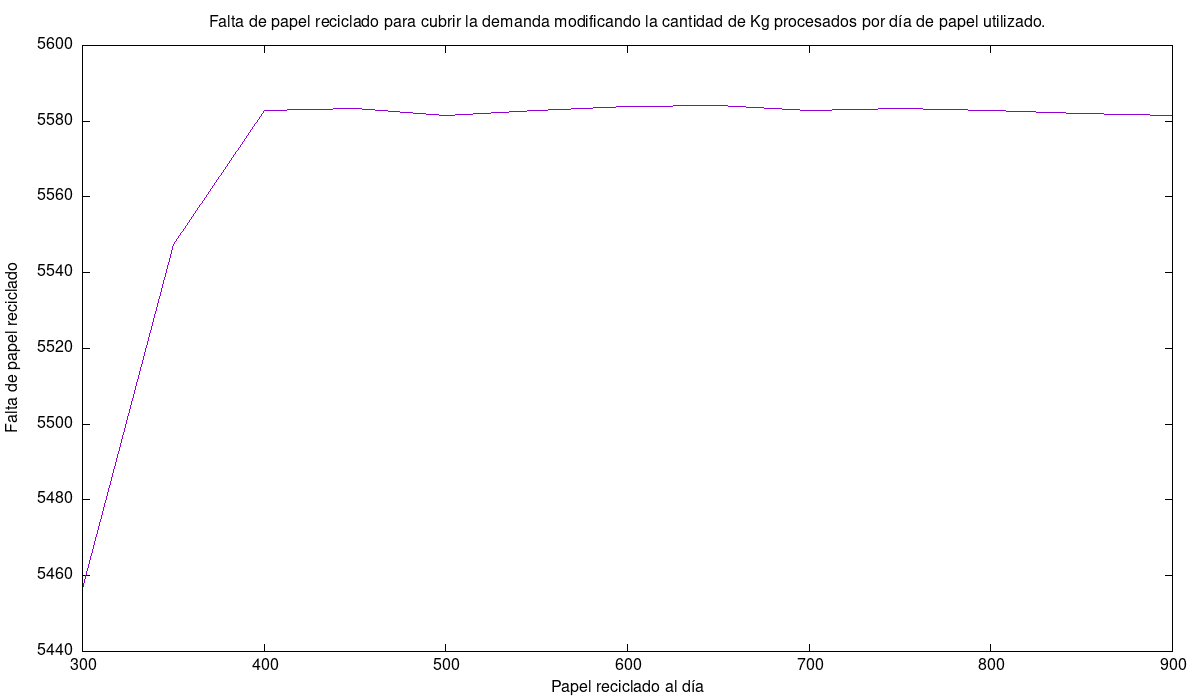
\includegraphics[width=\textwidth]{falta_papel_cambiando_kg_procesados.png}
	\caption{Modificando el número de Kg procesados cada día.}
\end{figure}


Como vemos no se llega a solucionar e incluso llega a empeorar, ya que es posible que muchos días la cantidad de papel en el contenedor rojo sea baja (si procesamos más papel en un día es mucho más probable que esto ocurra), haciendo que si un día llega poco papel, pero la demanda es alta, se sigue sin cubrir toda la demanda de papel reciclado, por ejemplo, si inicialmente tenemos 300Kg en el contenedor rojo, los procesamos teniendo 100Kg en el contenedor verde, si vendemos más de 100Kg (150 por ejemplo) y al siguiente día nos llegan tan solo 150Kg generando 50Kg, ya estaríamos perdiendo el primer día 50Kg y el segundo día, con suerte mantendríamos 20Kg, pero en cualquier otro caso perderíamos otros 10Kg en el mejor de los casos.

Por este motivo, para mejorar la falta de papel lo que habría que hacer es mejorar el método por el que se obtiene el papel reciclado, haciendo que se obtenga más papel reciclado con menos papel utilizado:

\begin{figure}[H]
  \centering
   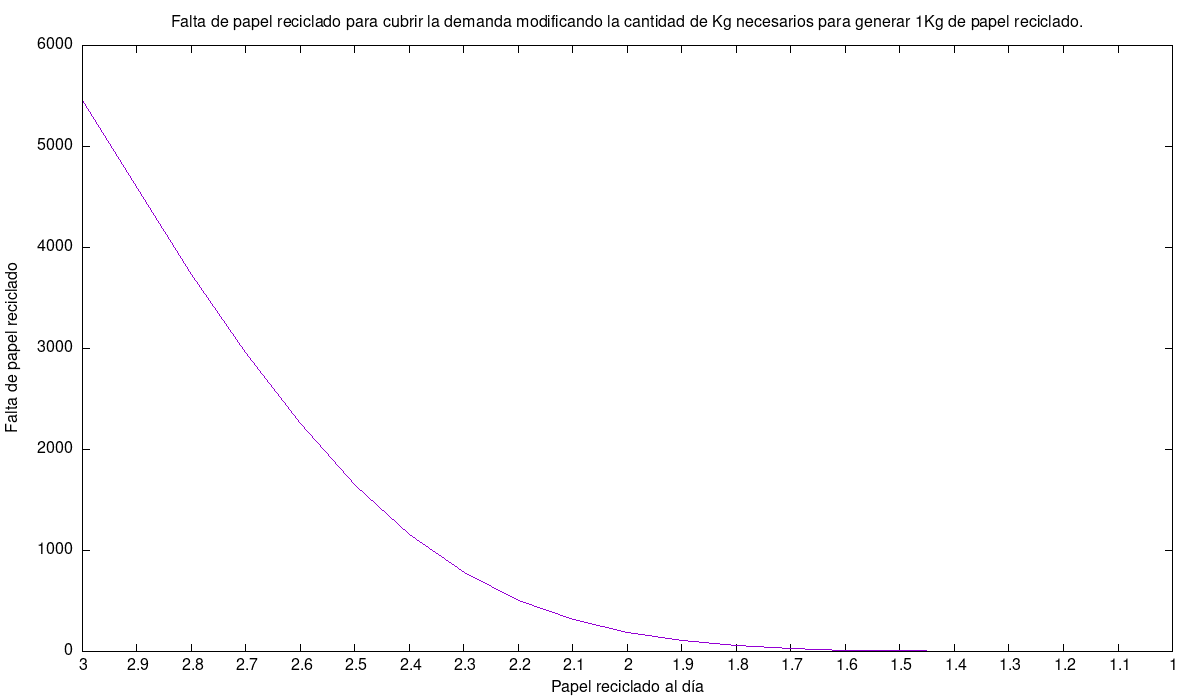
\includegraphics[width=\textwidth]{falta_papel_cambiando_proporcion_generacion.png}
	\caption{Modificando el número de Kg necesarios para obtener un Kg de papel reciclado.}
\end{figure}


En este caso vemos como si llegamos a suplir siempre la demanda ya que si hacemos el método de reciclaje muy optimo y aprovechamos casi todo el papel, aunque obtengamos pocos kilogramos de papel usado seremos capaces de mantener el papel reciclado que generamos.



% \begin{thebibliography}{9}
%
%
% \end{thebibliography}

\end{document}
